\chapter{\LaTeX Usage For Design For ECE}
\label{chapter:latexUsage}
\graphicspath{ {./chapter01/Fig} }

\begin{itquote}
The journey of a thousand miles begins with one step.
\end{itquote}

I can't be the only one.  I say this as I struggle to convert a textbook written
in Microsoft Word to \LaTeX and post it on GitHub.  There must be other faculty
members who have created quality content they want to share.
So this text is an Open Education Resources, free to use under the Creative
Commons license.  But how can we take advantage of deep reservoir of 
knowledge the community of senior design faculty have created over the
years.   In taking this particular project on, I want to move a step
towards the solution.

By hosting this textbook on Github, I want to encourage others to contribute 
their insights and ideas into our text.  For example, some of the processes in
this text are outdated. If that annoys you, then go to \\
\url{https://github.com/coulston/Design-For-Electrical-and-Computer-Engineering}\\
,the textbook repository,
fork, clone, make a branch, make your changes and
then do a pull request to merge them into the existing text.  If that sounds a 
bit overwhelming, don't worry, I plan on writing a chapter 2 to this how-to
to walk you through it.  The world is an imperfect place, I want you to be 
empowered to make it better.

\section*{Learning Objectives}
\noindent\rule{\linewidth}{1pt}
By the end of this chapter, the reader should:
\begin{itemize}
\item 	Understand some of my motivations in this project.
\item 	Understand the general philosophy of writing \LaTeX for this text.
\item Know how to create common structures like table, figure, examples.
\item Know how to use the Example environment.
\item Know how to create references to structures.
\end{itemize}

\section{Tables}
\label{section:howToTables}
When deciding on a methodology to implement some text formatting question,
my preference is to work with the existing \LaTeX packages before adding new
packages because every additional package adds additional time to build the
text.  All things being equal, I will always prefer a Minimum Working Example 
(MWE) over something more complex.  As a consequence of these two preferences,
when you inevitably need to search for a way to complete some text formatting
goal, I generally preface "MWE" in front of the thing I am trying to accomplish.

While tables are an incredibly important tool to communicate a lot of information 
in a structured format, they can be a challenge to tame.  As a result, I'll introduce
Table~\ref{table:thisIsTheFirstTable} as an example.  The \LaTeX code for this table
is shown below.

The following are some of the non-standard commands used in tables throughout the text.  I'd appreciate if you would 
edit this document to introduce new table features you might need to add with your content.  
\begin{enumerate}
\item \verb+rowcolor+
\item \verb+multicolumn+
\item \verb+hhline+
\item \verb+multirow+
\item \verb+makecell+
\end{enumerate}

\begin{table}[h]
\caption{Selection criteria for a ECE senior design textbook.}
\label{table:selectionCriteria}
\begin{tabular}{|m{2.5cm}|m{1.2cm}|m{2.8cm}|m{2.8cm}|m{2.8cm}|} \hline
\rowcolor{Gray}
 		& & \multicolumn{3} {c|} {Alternatives} \\ \hhline{|~|~|-|-|-|}
\rowcolor{Gray}
 \multirow{-2}*{Criteria} & \multirow{-2}*{Weights}  & Design for ECE & Ulysses &  Goodnight Moon\\ \hline
Relevance to class 			& 0.4 & 0.40 & 0.20 & 0.40 \\  \hline
Depth  						& 0.2 & 0.40 & 0.30 & 0.30 \\ \hline
Additional Resources  		& 0.2 & 0.40 & 0.30 & 0.30 \\ \hline
Length 						& 0.1 & 0.45 & 0.20 & 0.35 \\ \hline
Bedtime reading				& 0.1 & 0.10 & 0.10 & 0.80 \\ \hline
\multicolumn{2}{|l|}{
	\makecell[l]{	Lots of text in a \\
					multicolumn requires \\
					makecell and linebreaks.}}
  		      & 0.8 & 0.1 & 0.1 \\ \hline
\multicolumn{2}{|l|}{
{\rotatebox[origin=c]{90}{ \textbf{ Notes }}}} &  
	This is the logical choice.     &       
	I think it ends where it begins??? &
	Great choice for younger students. \\ \hline
\end{tabular}
\end{table}


\section{Figures}
\label{section:howToTables}

Thankfully figures are a lot easier to incorporate into \LaTeX if you follow a few simple rules.
\begin{enumerate}
\item Store all artwork in folder called ``Fig'' located in the chapter directory.
\item Convert all images to PDF format. This will eliminate needing additional packages to process different formats.
\item Include \verb+\graphicspath{ {./chapter01/Fig} }+ at the top of your \verb+chapter.tex+ file.
	This will insure that the path to your graphics file
\end{enumerate}

With this, let's admire Figure~\ref{table:bookPhilosophy}. 

\begin{figure}[h]
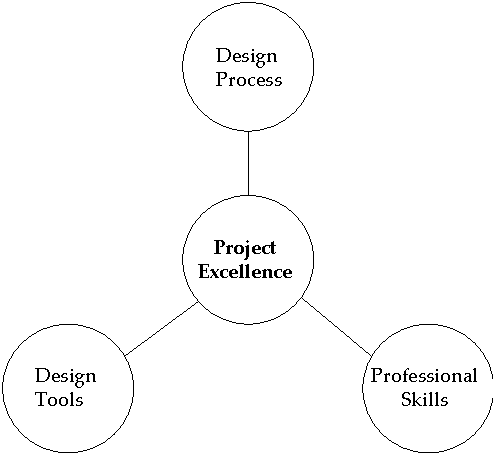
\includegraphics[width=2.9in,height=2.6in]{image7}

\caption{The guiding philosophy of this book. In order to
achieve success in executing engineering and design projects, it takes
an understanding of the design process, strong technical design tools,
and professional skills.}
\label{table:bookPhilosophy}
\end{figure}

The only exception to this simple format is when you want to include
several different images in the same figure frame.  When you do this
you will need to use the hspace command to stop all the images
from being squished next to one another.

\begin{figure}[h]
\hspace{1cm}

\includegraphics[width=1cm]{cc-logo}
\hspace{1cm}

\includegraphics[width=1cm]{cc-by}
\hspace{1cm}

\includegraphics[width=1cm]{cc-nc}
\hspace{1cm}

\includegraphics[width=1cm]{cc-sa}
\caption{(a) .}
\label{figure:howToCommonCollectiveLicense}
\end{figure}

\section{Equations}
\label{section:howToEquations}

Being a design textbook, I didn't think that there would be many equations.  Boy, was
I wrong.  The chapter on reliability was chock-full of equations.  Thank goodness, \LaTeX
is a master of equations.  So writing them will be one of the more plesant and straightforward
tasks. For example, let's look at Equation~\ref{equ:simpleEquation}.

\begin{equation}
\label{equ:simpleEquation}
x = \int v(t) dt
\end{equation}

Notice the reference to "equation" starts with a captial letter "E".  Not all equations will
need a number, in which case use the \$\$ delimiters when you want the equation to
float centered in the page.  For in-line equations use a single \$ at the start and end
of the equations.  Pretty standard \LaTeX stuff.

\section{Examples}
\label{section:howToExamples}

I wanted the examples to standout in the text.  The \verb+example+ environment allows
you to put a numbered, referencable, example in a shaded box.  Most examples will have
a problem and solution.  When they do, put these terms in bold.

\begin{example}{A Simple Example}
\label{example:aSimpleExample}
\emph{\textbf{\ul{Problem:}}} Choosing a senior design textbook for ECE. \\	% Force line break for spacing
\noindent\emph{\textbf{\ul{Solution:}}} Look at a bunch of textbooks and 
consider a variety of factors.  It is a very individual decision.
\end{example}

\section{Linking}
\label{section:howToLinking}
The use of links inside and outside the document are an important feature.  The use
of descriptive names in your label commands is a good start.  As best practice, use
the following format for your labels.  And remember, you need to put the 
\verb+\label+ \ul{after} any associated captions.

\begin{verbatim}
	\label{<type>:<chapterName><description>
\end{verbatim}

The \verb+chapterName+ and \verb+desciption+ should be self explanatory.  I tend to 
try to summarize both rather than being to verbose.  I have tried to standardize the 
\verb+<type>+ field to one of the following:
\begin{itemize}
\item  table, like for Table~\ref{table:selectionCriteria}
\item  figure, like for Figure~\ref{table:bookPhilosophy}
\item equation
\item example
\item section
\item chapter
\end{itemize}

Use external links to point readers to an important resource like the US Bureau of Labor Statistics, 
\url{http://stats.bls.gov}. Note, some URLs can get quite long, so be prepared to introduce some line 
breaks before and after URL references.

\section{Summary and Further Reading}
\label{section:summary-and-further-reading}
Thanks for tking the time to review this How-To guide.  I appreciate your contributions to the text and any of the 
associated materials.
